% Édito
\part*{Edito}

\begin{figure}[H]
    \center
    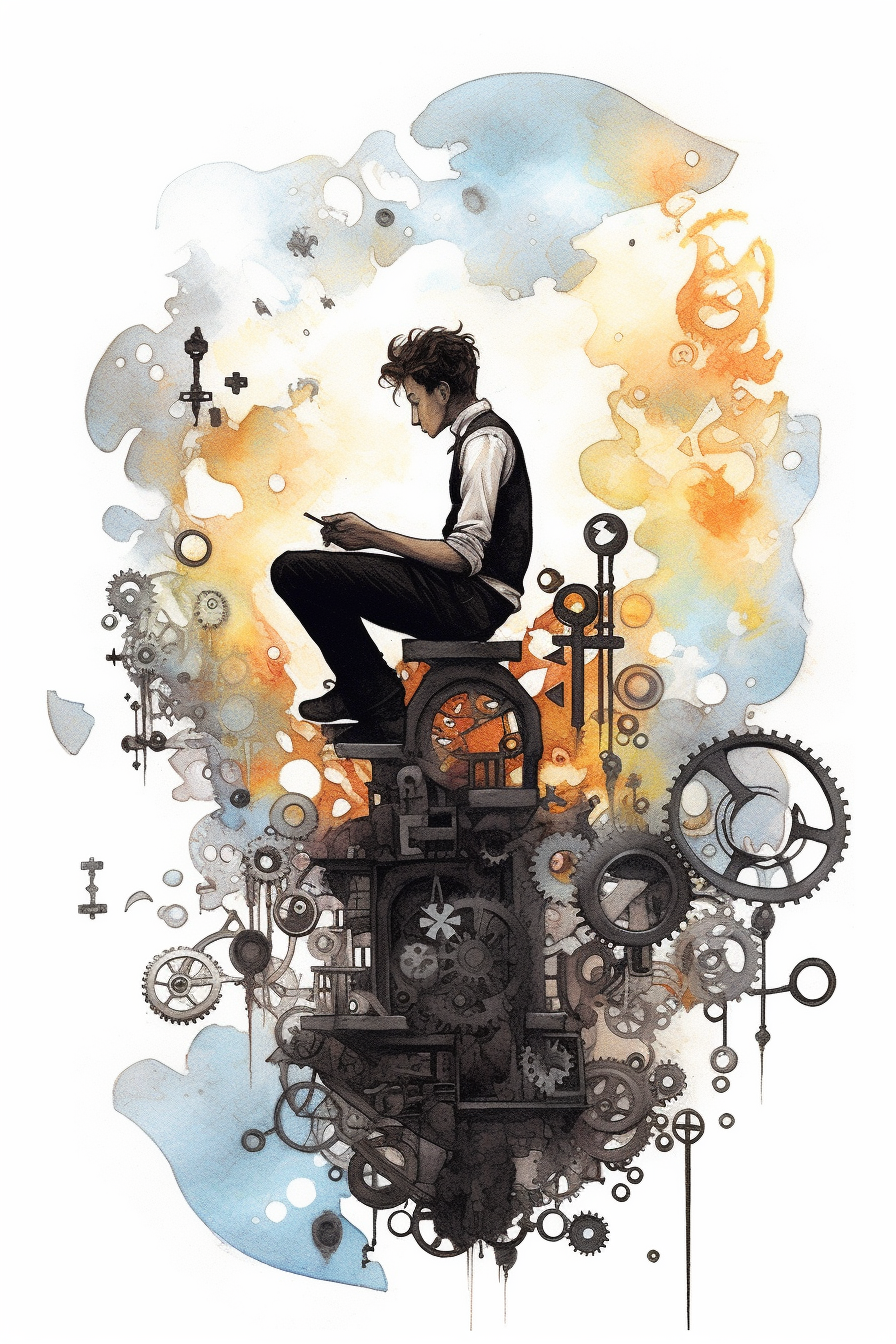
\includegraphics[keepaspectratio, width=\textwidth]{images/19e9e263-d40a-4bd0-bf6d-5aded7ffb396.png}
\end{figure}

Je me souviens encore de mes débuts en tant que développeur. Fraîchement diplômé, plein d'énergie et d'enthousiasme, prêt à plonger dans le monde de la programmation et à faire ma marque. Je me sentais invincible, armé de mes connaissances en informatique et de ma passion pour le code. J'étais prêt à affronter le monde.

Et puis, la réalité a frappé.

Je me suis retrouvé face à face avec un mur imposant et apparemment insurmontable. Ce mur avait un nom : l'expérience professionnelle. Partout où je postulais, la même demande résonnait encore et encore - "recherche développeur junior avec expérience".

C'était un paradoxe qui me rendait perplexe. Comment un jeune développeur, tout juste sorti de l'école, pourrait-il avoir une expérience professionnelle significative ? Et pourtant, cette exigence semblait être la norme, une sorte de rite de passage que chaque développeur devait traverser.

Malgré cette difficulté qui me paraissait insurmontable, j'ai réussi à trouver mon premier emploi et à faire mes armes au sein d'un éditeur de logiciel.

J'ai commencé à faire du bénévolat dans des écoles de formation en informatique, comme EDEN school\footnote{EDEN School est la seule école de formation en développement informatique web après la classe de 3ème. Pour en savoir plus, consultez le site web : \href{https://www.edenschool.fr}{ \textcolor{blue}{https://www.edenschool.fr} }}, où j'ai eu l'occasion de côtoyer de jeunes développeur·euse·s qui rencontraient les mêmes difficultés que moi à leurs débuts de carrière. Leurs histoires, leurs luttes et leurs succès m'ont inspiré·e à écrire ce livre, dans l'espoir d'aider d'autres jeunes développeur·euse·s à surmonter les obstacles qui se dressent sur leur chemin.

Ce livre est le fruit de mon propre voyage en tant que développeur, des leçons que j'ai apprises, des erreurs que j'ai commises, des succès que j'ai remportés. Il s'inspire également des expériences et des sagesses de nombreux autres développeur·euse·s que j'ai eu le privilège de rencontrer et de travailler avec tout au long de ma carrière.

À travers les chapitres de ce livre, nous explorerons ensemble les différentes étapes du parcours d'un·e jeune développeur·euse pour acquerir de l'expérience. Nous discuterons de l'importance de contribuer à l'open source, de développer des projets personnels, de réseauter professionnellement, d'apprendre de manière efficace et continue, et de nombreux autres sujets essentiels.

J'espère que ce livre vous sera utile, que vous soyez un·e étudiant·e en informatique cherchant à décrocher son premier stage, un·e jeune développeur·euse luttant pour trouver son premier emploi, ou même un·e développeur·euse plus expérimenté·e cherchant à affiner ses compétences et à progresser dans sa carrière.

En fin de compte, rappelez-vous ceci : la quête de l'expérience est une quête sans fin. Il y aura toujours quelque chose de nouveau à apprendre, un défi à relever, une compétence à maîtriser. Mais avec les bonnes attitudes, une volonté d'apprendre et une détermination à réussir, vous pouvez et vous surmonterez les défis qui se présentent à vous.

Bonne chance dans votre quête, jeune développeur·euse.


